\documentclass{beamer} % [aspectratio=169]
\usetheme{ucl}
\setbeamercolor{banner}{bg=brightblue}
\setbeamersize{description width=2em}
\setbeamertemplate{navigation symbols}{\vspace{-2ex}} 

%\usepackage{fontspec}
\usepackage[utf8]{inputenc}
% \usepackage[english, greek]{babel}

\usepackage{caption}
\usepackage[T1]{fontenc} % Turn £ into $
\usepackage{minted}
\usemintedstyle{emacs}

\usepackage{fancyvrb}
\usepackage{xcolor}
\usepackage{url}

\usepackage{natbib}
\usepackage{bibentry}
\usepackage{url}


\usepackage{tikz}
\usetikzlibrary{positioning} 
\usetikzlibrary{shapes,arrows}

\usepackage{tikz-uml}

\tikzset{
  font={\fontsize{9pt}{12}\selectfont}}



\newcommand\emc[1]{\textcolor{brightblue}{\textbf{#1}}}

\AtBeginSection[]{
  \begin{frame}
  \vfill
  \centering
  \begin{beamercolorbox}[sep=8pt,center,shadow=true,rounded=true]{title}
    \usebeamerfont{title}\insertsectionhead\par%
  \end{beamercolorbox}
  \vfill
  \end{frame}
}

\author{Prof.\ George Danezis, University College London, UK}
\title{Computing \& Visualization}
\subtitle{ENGS102P: Design and Professional Skills }
% \institute{}
\date{Term 1, 2017}


\begin{document}
\nobibliography*


\frame{
\titlepage
}

\begin{frame}
\frametitle{Introducing Computing Visualization}

\begin{itemize}
  \item \emc{Engineering}: \\ UML use case diagrams, UML sequence diagrams, flow diagrams.
  \item \emc{Scientific}: \\ graphs \& data, architecture and data flow diagrams, ...   
  \item \emc{End-user}: \\ Web pages layout \& fonts, visuals, colours, ...
\end{itemize}

\end{frame}

\section{Engineering Visualization}


\begin{frame}
\frametitle{Use-cases}

\begin{block}{Requirements Engineering}
Use cases allow system designers to capture ways in which actors may use the system. 
\end{block}

\begin{itemize}
  \item \emc{Actors are beneficiaries} of the system.
  \item Different types of actors may make different uses of the system.
  \item Use-cases capture \emc{`what'} happens, but abstract \emc{`how'}.
  \item Use cases may \emc{include} other \emc{reusable} use-cases.
  \item Use cases may \emc{extend} others, to \emc{specialize} them..
\end{itemize}

\vspace{3mm}
Standard diagrams using the Unified Modeling Language (UML).

\end{frame}

\begin{frame}

\frametitle{How to capture requirements?}

\emc{Talk to users!} Capture \emc{user stories} in the format:

\begin{center}
 \small \texttt{As a < type of user >, \\ I want < some goal > \\ (so that < some reason >).}
\end{center}

\vspace{3mm}
Example user stories:
\begin{itemize}
  \item As a blog author, I want to post a story, so that readers can read it.
  \item As a blog reader I want to read stories.
  \item As a blog admin I want to moderate stories, so that I filter profanities.
\end{itemize}

\end{frame}


\begin{frame}

\frametitle{UML Use-case diagram}

\begin{center}
\begin{tikzpicture}
\begin{umlsystem}[x=4, fill=red!10]{The blogging system}
\umlusecase{Create \& Edit Story}
\umlusecase[y=-2]{Submit Story}
\umlusecase[y=-4]{Approve Story}
\umlusecase[x=3.2, y=-4]{Read Story}
%\umlusecase[x=6, fill=green!20]{use case5}
%\umlusecase[x=6, y=-4]{use case6}
\end{umlsystem}

\umlactor{Author}
\umlactor[y=-4]{Admin}
\umlactor[x=10.2, y=-4]{Reader}

% \umlinherit{Admin}{Author}
\umlassoc{Author}{usecase-1}
\umlassoc{Author}{usecase-2}
\umlassoc{Admin}{usecase-3}
\umlassoc{Reader}{usecase-4}
%\umlassoc{admin}{usecase-5}
%\umlassoc{admin}{usecase-6}
%\umlinherit{usecase-3}{usecase-2}
%\umlVHextend{usecase-5}{usecase-4}
%\umlinclude[name=incl]{usecase-3}{usecase-4}

%\umlnote[x=7, y=-7]{incl-1}{note on include dependency}
\end{tikzpicture}
\end{center}

\end{frame}


\begin{frame}

\frametitle{UML Use-case diagram: inherit, include \& extend.}

\begin{center}
\begin{tikzpicture}
\begin{umlsystem}[x=5, fill=red!10]{The blogging system}
\umlusecase[name=CrEd]{Create \& Edit Story}
\umlusecase[name=SS, y=-2]{Submit Story}
\umlusecase[name=AS, y=-4]{Approve Story}
\umlusecase[name=L, x=5, y=-2]{Login}
\end{umlsystem}

\umlactor{Author}
\umlactor[y=-4]{Admin}

\umlinherit{Admin}{Author}
\umlassoc{Author}{CrEd}
\umlassoc{Author}{SS}
\umlassoc{Admin}{AS}
\umlextend[name=nadmin]{SS}{AS}
\umlinclude{CrEd}{L}
\umlinclude{SS}{L}

\umlnote[x=9, y=-4]{nadmin-1}{If Administrator}
\end{tikzpicture}
\end{center}

\end{frame}


\begin{frame}

\frametitle{Agile User Story boards: using physical post-it notes}

\center
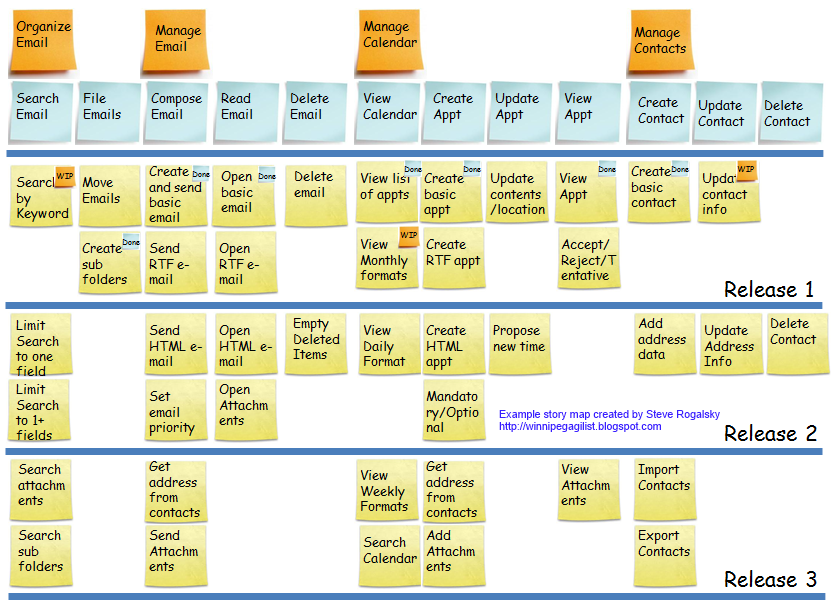
\includegraphics[width=9cm]{assets/UserStoryMap}

\tiny Graphic from \url{http://winnipegagilist.blogspot.com/2012/03/how-to-create-user-story-map.html}.

\end{frame}

\begin{frame}

\frametitle{UML Sequence Diagrams}

Complex computing systems are composed of \emc{components} that interact with each other in \emc{sequences} of steps. 

\vspace{3mm} UML Sequence diagrams capture sequences of operations that perform an action.

\begin{block}{Example: Writing to redundant storage}
When information needs to persist, despite failures, it is customary to write to multiple databases, on different disks. However, writing to disk takes time so some operations can tolerate just persisting in memory. How to depict this operation using a sequence diagram?
\end{block}

\end{frame}

\begin{frame}

\begin{center}
\begin{tikzpicture}
\begin{umlseqdiag}[font=\small]

\umlactor[class=U, scale=0.5]{user}
\umlobject[class=W, x=3]{writer}
\umldatabase[scale=0.5, class=DB, x=6, fill=blue!20]{db0}
\umldatabase[scale=0.5, class=DB, x=8, fill=blue!20]{db1}


\begin{umlcall}[op={write(v,t)}, type=synchron, return=ok]{user}{writer}

\begin{umlfragment}[type=alt, label={t=memory}, inner xsep=10, fill=green!10]
\begin{umlcallself}[op=cache(v), type=synchron, return=ok]{writer}
\end{umlcallself}
\umlfpart[{t=disk}]
\begin{umlcall}[op=commit(v), type=synchron, fill=red!10, return=ok]{writer}{db0}
\end{umlcall}
\begin{umlcall}[op=commit(v), type=synchron, fill=red!10, return=ok]{writer}{db1}
\end{umlcall}

\end{umlfragment}

\end{umlcall}

\end{umlseqdiag}
\end{tikzpicture}
\end{center}

\end{frame}

\begin{frame}

\frametitle{Visual representation of algorithms.}

In 1972, Dahl, Dijkstra and Hoare publish \emc{structured programming}:
\begin{itemize}
  \item Programs are sequences of \emc{statements} (rectangles).
  \item Control flow can branch on \emc{conditions} (diamonds).
  \item Control flow can go back or forward to denote \emc{loops} (circle)
  \item Ban: \texttt{goto} statements, and multiple entries or exits in functions.
\end{itemize}

\vspace{3mm}
\emc{Control flow diagrams} are used to this day to illustrate how algorithms work.
\begin{itemize}
  \item Not used for actual implementation or documentation.
  \item Some restrictions are lifted: \texttt{continue}, \texttt{break}, exceptions.
  \item Real-world \texttt{C} programs use \texttt{goto} for error handling.
\end{itemize}

\end{frame}

\begin{frame}

\frametitle{Control flow diagram for euclid's algorithm.}

% Define block styles
\tikzstyle{joinx} = [circle, draw, fill=blue!20,
    text width=0.5em, text badly centered, node distance=1.2cm, inner sep=0pt]

\tikzstyle{decision} = [diamond, draw, fill=blue!20, shape aspect=2.7,
    text width=4.5em, text badly centered, node distance=1.2cm, inner sep=0pt]
\tikzstyle{block} = [rectangle, draw, fill=blue!20, 
    text width=5em, text centered, rounded corners, minimum height=2em]
\tikzstyle{line} = [draw, -latex']
    
\begin{center}
\begin{tikzpicture}[node distance = 1.2cm, auto]
    % Place nodes
    \node [block] (init) { {euclid($a$,$b$)} };
    \node [joinx,below of=init] (while) {};
    \node [decision, below of=while] (wcond) {$a \neq b$};
    \node [decision, right of=wcond, node distance=3cm] (ifcond) {$a > b$};
    \node [block, right of=ifcond, node distance=3cm] (a) {$a = a - b$};
    \node [block, below of=a] (b) {$b = b - a$};
    \node [block, below of=wcond, node distance=2.4cm] (ret) {return $a$};

    % Draw edges
    \draw [line] (init) -- (while);
    \draw [line] (while) -- (wcond);
    \draw [line] (wcond) -- (ret) node [midway, left] {F};
    \draw [line] (wcond) -- (ifcond) node [midway] {T};
    \draw [line] (ifcond) -- (a) node [midway] {T};
    \draw [line] (ifcond) |- (b) node [midway, left] {F};
    \draw[->] (b) -- node {} ++(2,0) |- (while);     
    \draw[->] (a) -- node {} ++(2,0) |- (while);

\end{tikzpicture}
\end{center}

\end{frame}

\begin{frame}

\frametitle{More on UML \& Production notes.}

We will study more types of UML diagrams later in the course:
\begin{itemize}
  \item UML \emc{class diagrams} capture the relationships between objects in a program.
  \item UML \emc{state diagrams} capture states in which a program can be in.
\end{itemize}

\vspace{3mm}
Production notes:
\begin{itemize}
  \item Ensure your diagrams are of \emc{print quality} by using vector graphics and rendering them in \texttt{postscript} (eps, ps) or \texttt{pdf}. Not bitmaps.
  \item Prefer to use \emc{text-based description languages} to build documents and graphics. Those can be folded under \emc{version control} (git), and can be tweaked and \emc{produced by programs}. 
  \item The example diagrams were drawn using \texttt{pdflatex}, with the \texttt{tikz-uml} package. Learn how to use \texttt{tikz}, it is a powerful tool.
\end{itemize}

\end{frame}


\section{Scientific Visualization}

\begin{frame}

\frametitle{Aims of Scientific Visualization.}

According to Edward Tufte (1983):
\begin{description}
\item[Clarity.] Lack of ambiguity and confusion.
\item[Precision.] Truthful results; Distortion‐free presentation.
\item[Efficiency.] Minimal ``chartjunk''
\end{description}

\vspace{5mm}
\begin{block}{Recommended Reading}
Tufte, Edward R. The Visual Display of Quantitative
Information; Graphics Press: Cheshire, CT, 1983; pp 1‐197
\end{block}

For excerpts see \url{http://cs.unm.edu/~pgk/IVCDs14/minitufte.pdf}

\end{frame}

\begin{frame}

\frametitle{Basic principles on visualizing quantitative information.}

Tufte's key principles.
\begin{itemize}
\item Show \emc{comparisons}.
\item Show \emc{causality}.
\item Show \emc{multivariate data}.
\item Integrating \emc{relevant evidence}.
\item \emc{Documentation}, methods and meta-data.
\item \emc{Content} counts most of all! 
\end{itemize}

\vspace{3mm}
For a historical overview see also `Envisioning Information' by E. Tufte.\\ 
\url{https://tinyurl.com/tufteEnvisioning}

\end{frame}

\begin{frame}

\frametitle{Introducing Graphs.}

Graphs depict relationships between two or more quantities.
\begin{center}
\includegraphics[width=8cm]{assets/entropy1}
\captionof{figure}{the relationship between quality of anonymity (entropy) and the rate of traffic in the Loopix anonymity system ($\lambda$), for different delay rates ($\mu$)}
\end{center}

\tiny From Ania M. Piotrowska, Jamie Hayes, Tariq Elahi, Sebastian Meiser, George Danezis:
The Loopix Anonymity System. USENIX Security Symposium 2017: 1199-1216

\end{frame}


\begin{frame}

\frametitle{Good scientific graphs (I).}

Best practices -- which ones are applied in the example?
\begin{itemize}
\item All information and meta-information must be \emc{correct}!
\item A \emc{title} summarizes \& a \emc{caption} describes it.
\item A \emc{legend} explains what different lines represent.
\item \emc{Font size is large} enough to read.
\item \emc{Axis} are labeled with the \emc{quantities}, and their \emc{units}.
\item \emc{Axis} have a numerical scale, and indicate if they are a \emc{log scale}.
\item Only related data points may be \emc{connected} by lines.
\item \emc{Data points are indicated}, and extrapolating lines obvious.
\item \emc{Error bars} indicate the standard derivation or error.
\item \ldots
\end{itemize}

\end{frame}

\begin{frame}

\frametitle{Good scientific graphs (II).}

Best practices -- which ones are applied in the example? (Continued)
\begin{itemize}
\item \ldots
\item All \emc{features are identified}.
\item They are unambiguous if \emc{rendered without color}.
\item A faint \emc{grid} to facilitate reading. 
\item \emc{High-resolution} in relation to medium.
\end{itemize}

\vspace{3mm}
\begin{block}{Pro tip: make scientific graphs using code.}
You will inevitably tweak the aesthetics of your graph, and also your data, more times than you care to re-work it by hand. For consistency, version control, and reproducibility use a programming language to make graphs, such as \texttt{matplotlib} in \texttt{Python}, or \texttt{d3.js} in \texttt{javascript.}
\end{block}

\end{frame}


\begin{frame}

\frametitle{Explanatory diagrams.}

Scientific works also contain non-quantitative \emc{explanatory diagrams}.

\vspace{5mm}
\begin{itemize}
\item Principles of \emc{clarity}, \emc{precision} and \emc{efficiency} apply. 
\item \emc{Architecture diagrams} present very high-level explanations.
\item \emc{Data flow diagrams} present mid- low-level explanations centered on data and operations on the data.
\end{itemize}


\end{frame}

\begin{frame}

\frametitle{An architecture diagram: SCION.}

\begin{center}
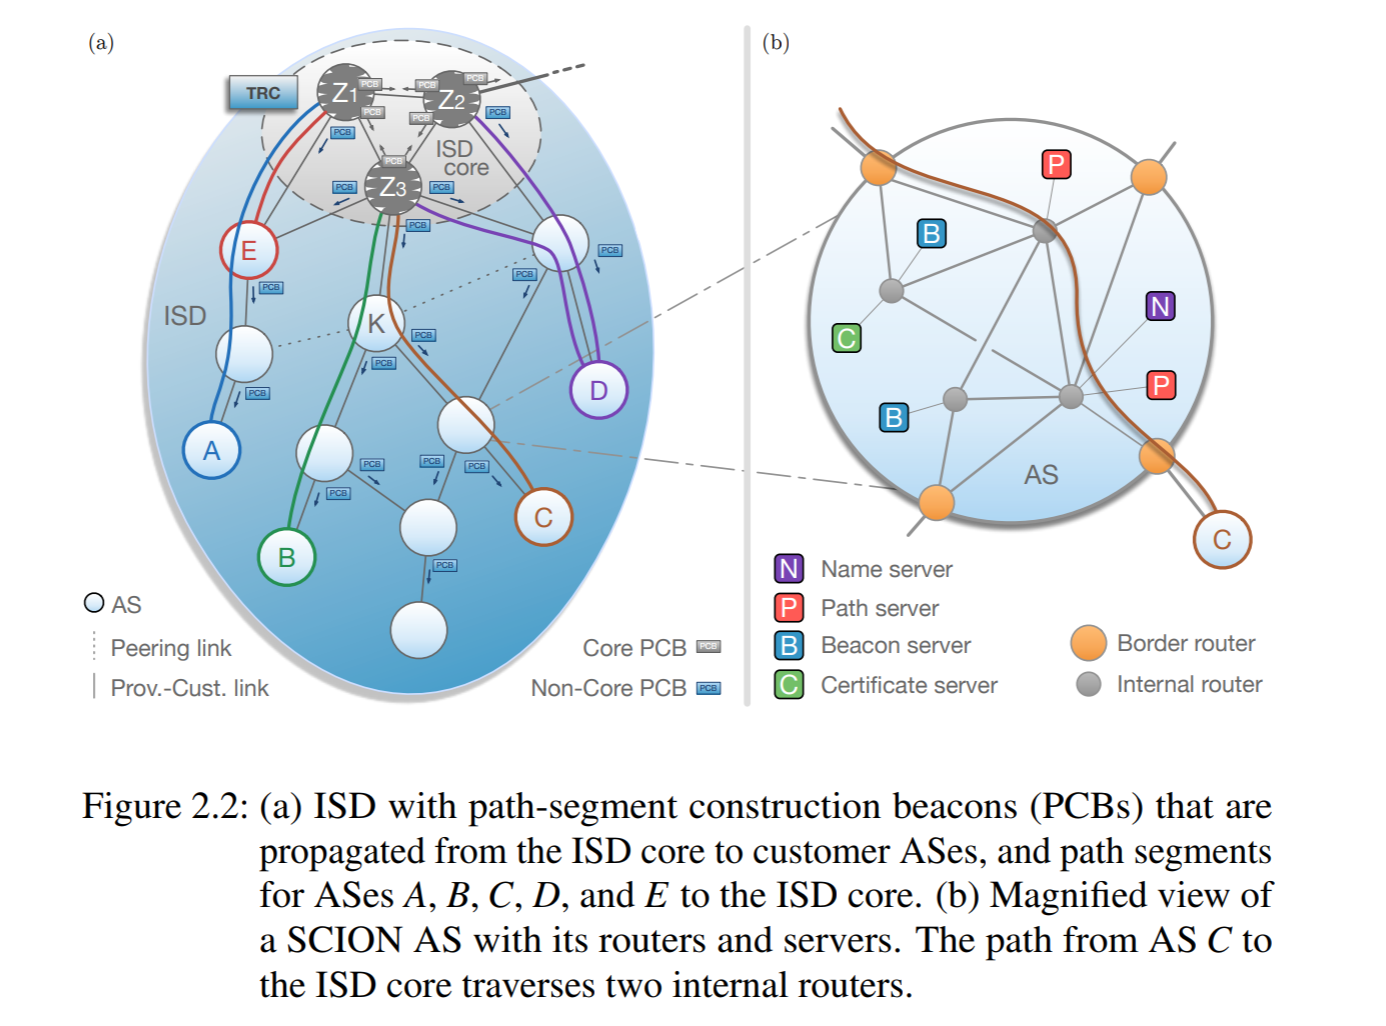
\includegraphics[width=8cm]{assets/scion}
\end{center}

\tiny From SCION: A Secure Internet Architecture. 
Adrian Perrig, Pawel Szalachowski, Raphael M. Reischuk and Laurent Chuat.
Publisher: Springer Verlag, August 2017.
\end{frame}

\begin{frame}

\frametitle{A data flow diagram: The AES-GCM encryption algorithm.}

\begin{center}
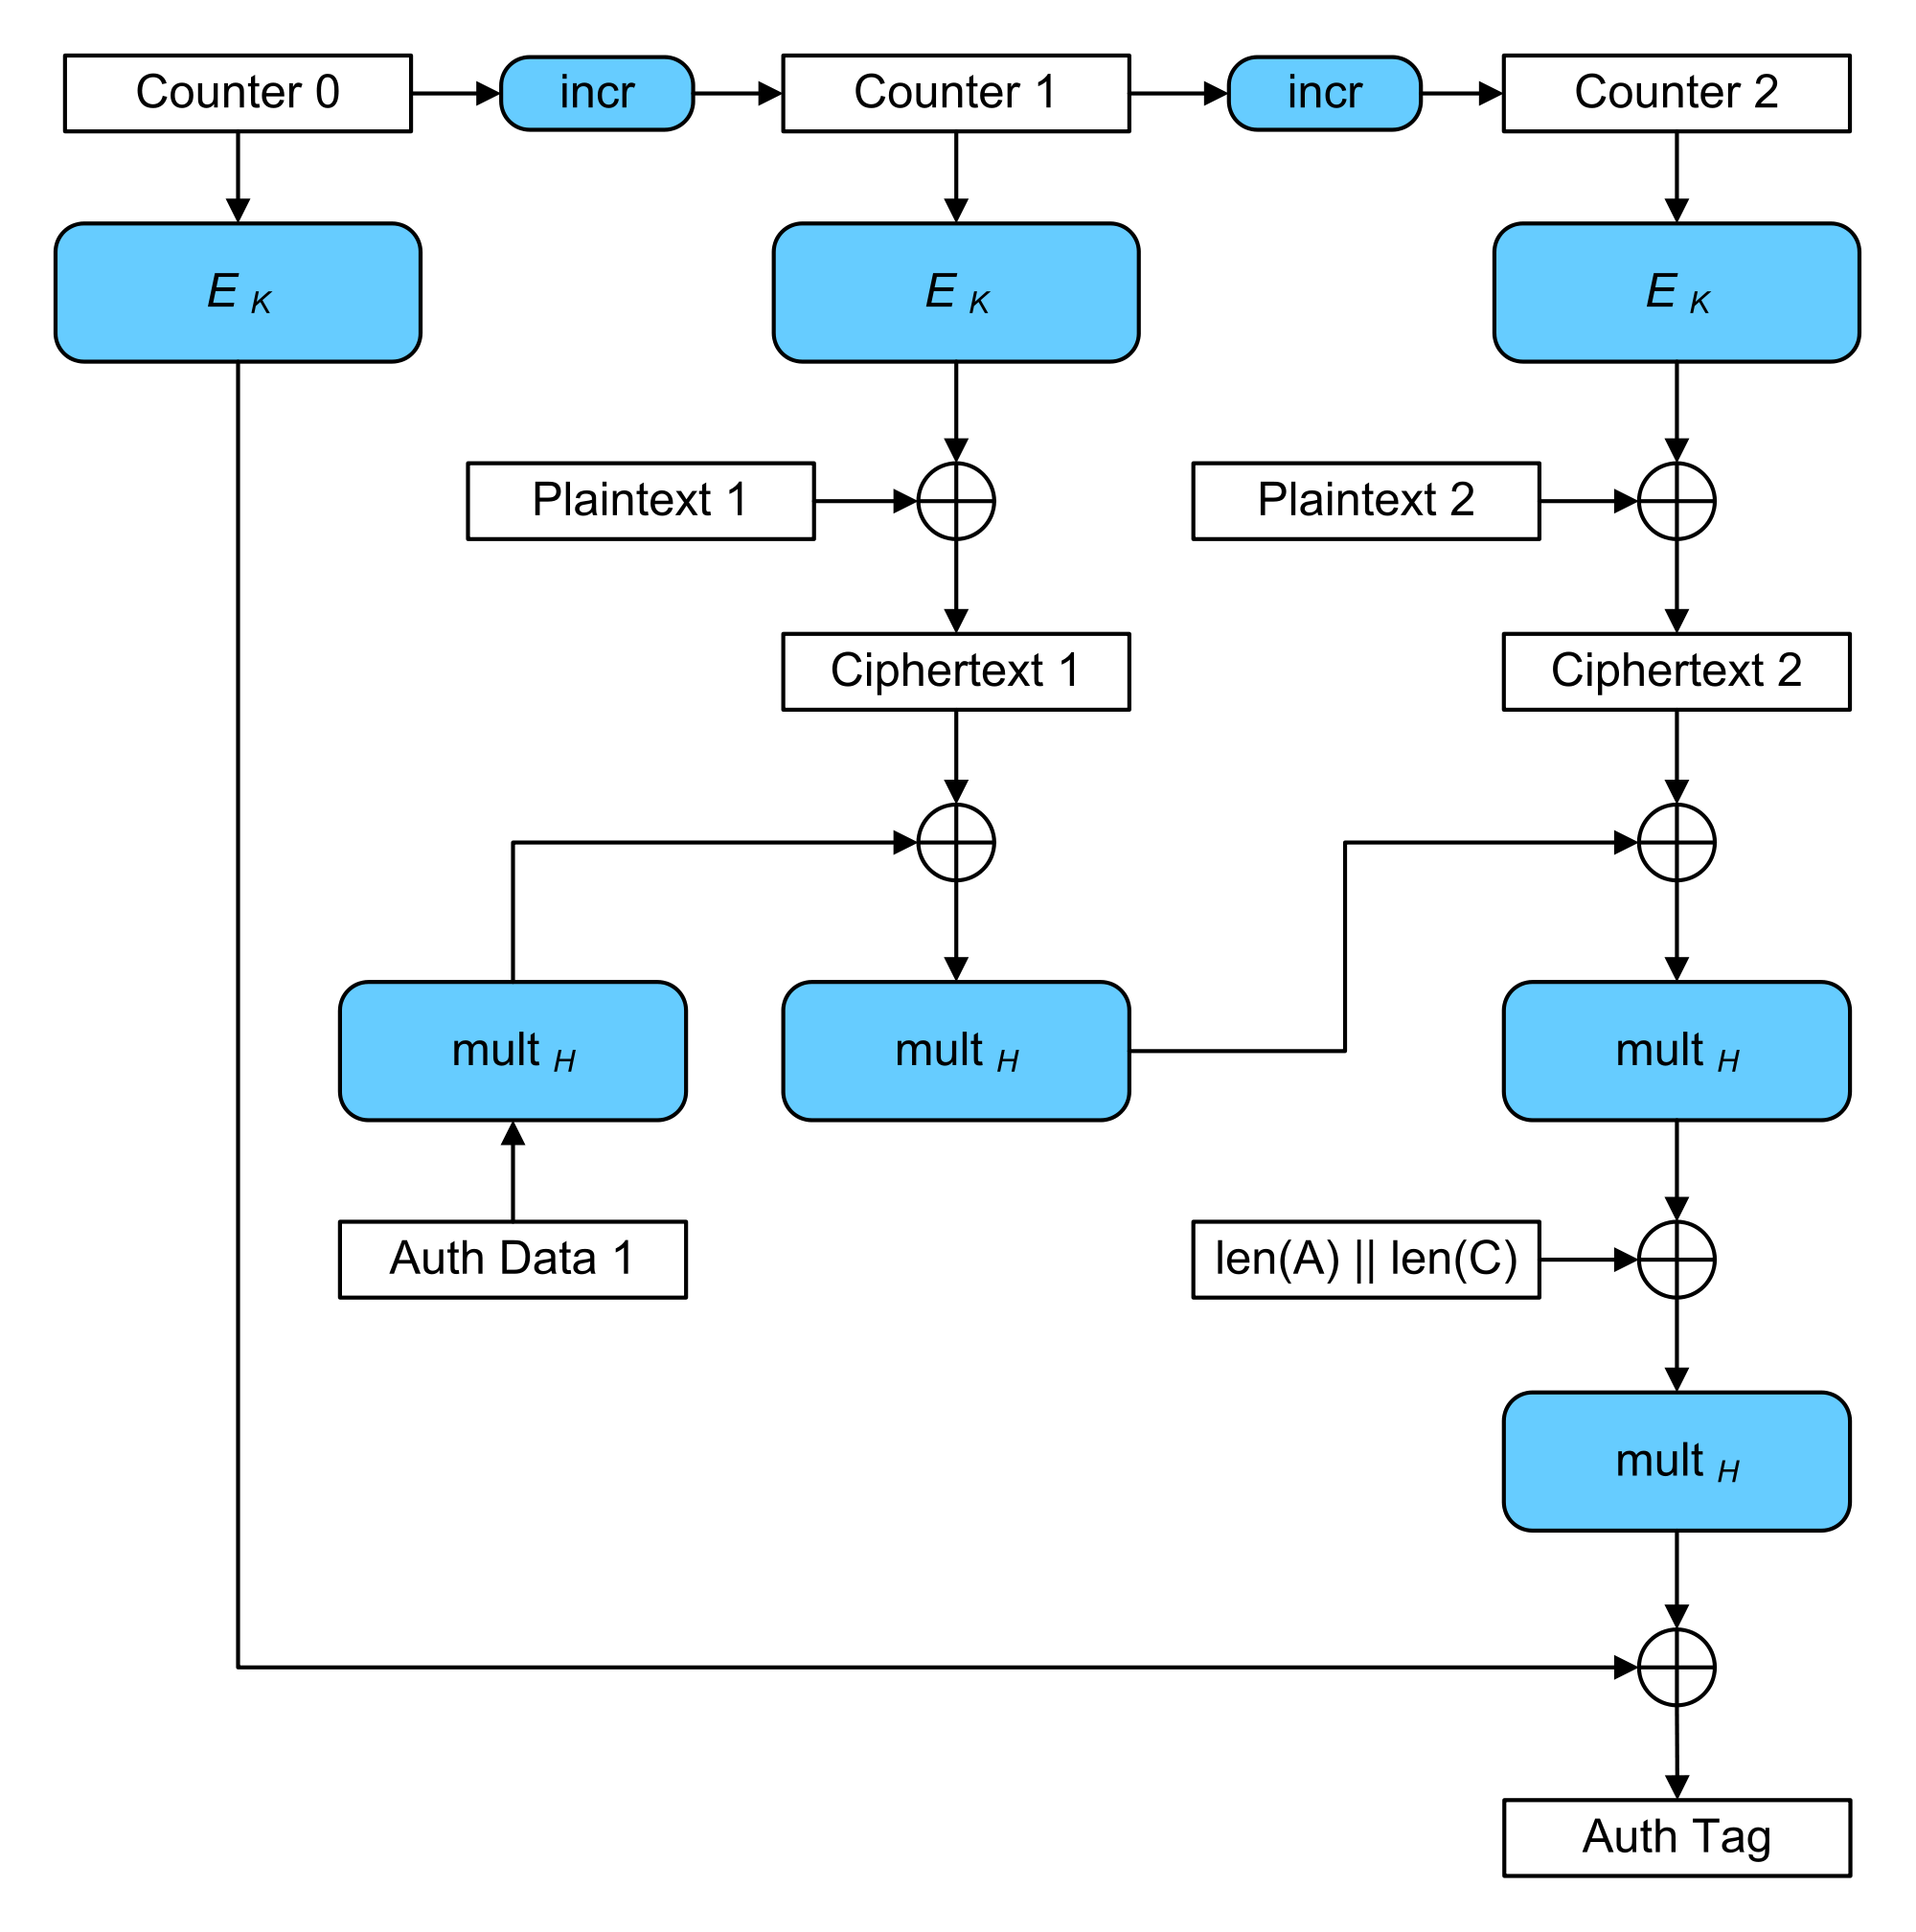
\includegraphics[width=6cm]{assets/GCM-Galois_Counter_Mode}
\end{center}

\tiny From \url{https://en.wikipedia.org/wiki/Galois/Counter_Mode}.
\end{frame}


\section{End-user Visualization}

\begin{frame}

\frametitle{`Demo or die' -- Nicholas Negroponte (MIT Media Lab)}

Demonstrating your work increases its \emc{impact}:
\begin{itemize}
  \item Always make an \emc{end-user demonstration} of what you build.
  \item The demo needs to be \emc{minimally functional}.
  \item Yet, it has to be \emc{visually attractive} and \emc{professional looking}.
\end{itemize}

\vspace{3mm}
Equip yourselves with \emc{quick prototyping} techniques to build \emc{beautiful things}.

\end{frame}

\begin{frame}

\frametitle{Elements of good visual style.}

Traditional \emc{graphic design} quality matters:
\begin{itemize}
  \item Clear and aesthetic \emc{layout}.
  \item Wise choice of \emc{colors}.
  \item Choice of \emc{font} to match aesthetics (typeface, style, size).
  \item \emc{Consistency} of the visual experience.
  \item Line, color, texture, shape, size, value \& space.
\end{itemize}

Modern \emc{interaction design} qualities also matter:
\begin{itemize}
  \item \emc{Intuitive} use and operation.
  \item \emc{Fluid} and responsive to environment and user actions.
  \item Effective at providing \emc{natural feedback} to user.
\end{itemize}

\end{frame}

\begin{frame}

\begin{center}
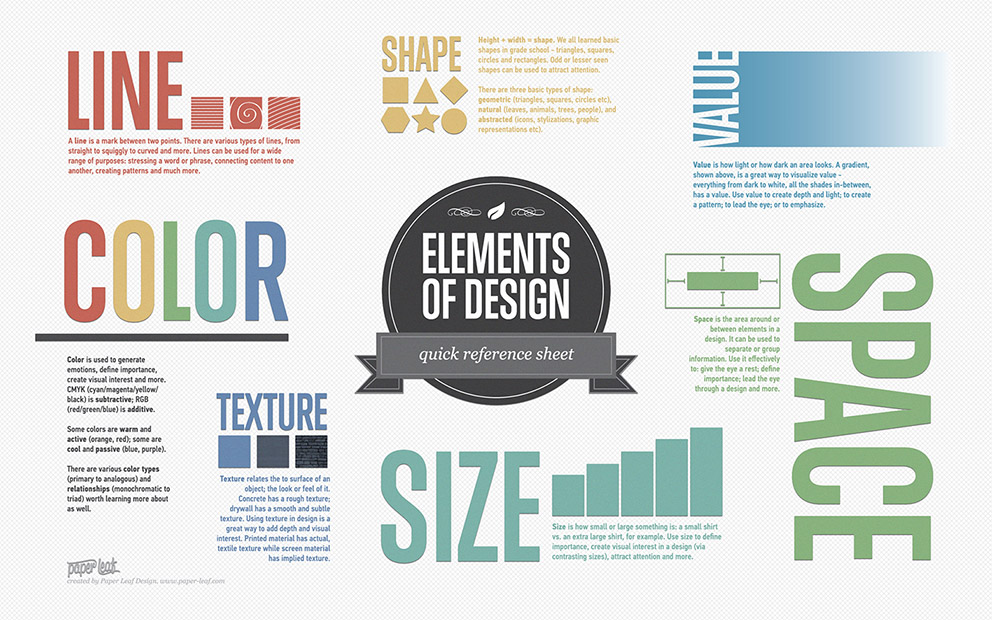
\includegraphics[width=11cm]{assets/Elements-of-Design2}
\end{center}

\tiny From \url{http://www.unahealydesign.com}.

\end{frame}

\begin{frame}

\frametitle{Quick prototyping \& great design.}

Advice: re-use what professional designers have created!
\begin{itemize}
  \item For web and mobile layouts use \emc{Bootstrap} and existing \emc{themes}.
  \url{http://getbootstrap.com/}
  \item Do not pick colors at random: use a \emc{color palette} generator.
  \url{http://paletton.com/}
  \item In in doubt about typeface, stick to \emc{Helvetica}. \\
  Or follow the \emc{How to choose a font} flow chart by Julian Hansen. 
  \url{http://www.julianhansen.com}
\end{itemize}

\end{frame}


\begin{frame}

\begin{center}
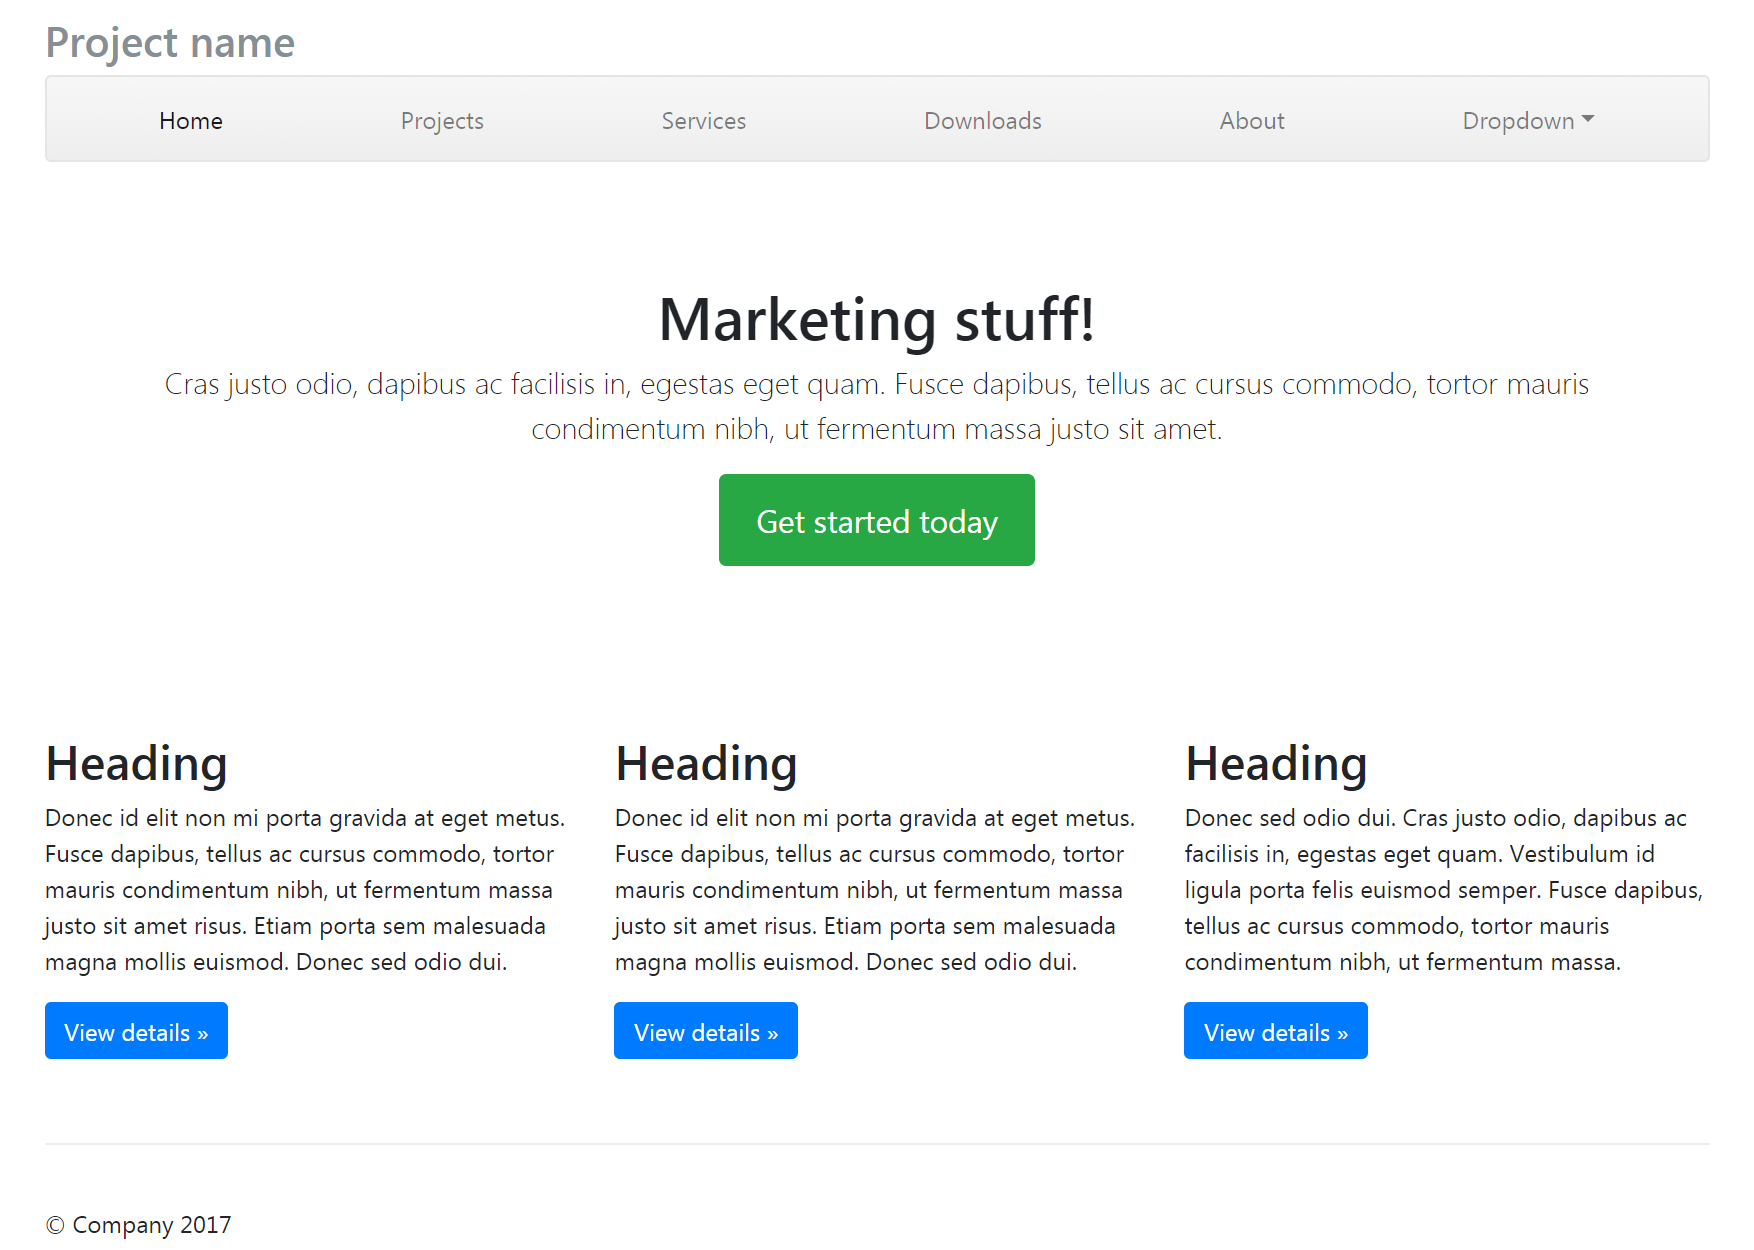
\includegraphics[width=11cm]{assets/bootstrap}
\end{center}

\end{frame}


\begin{frame}

\begin{center}
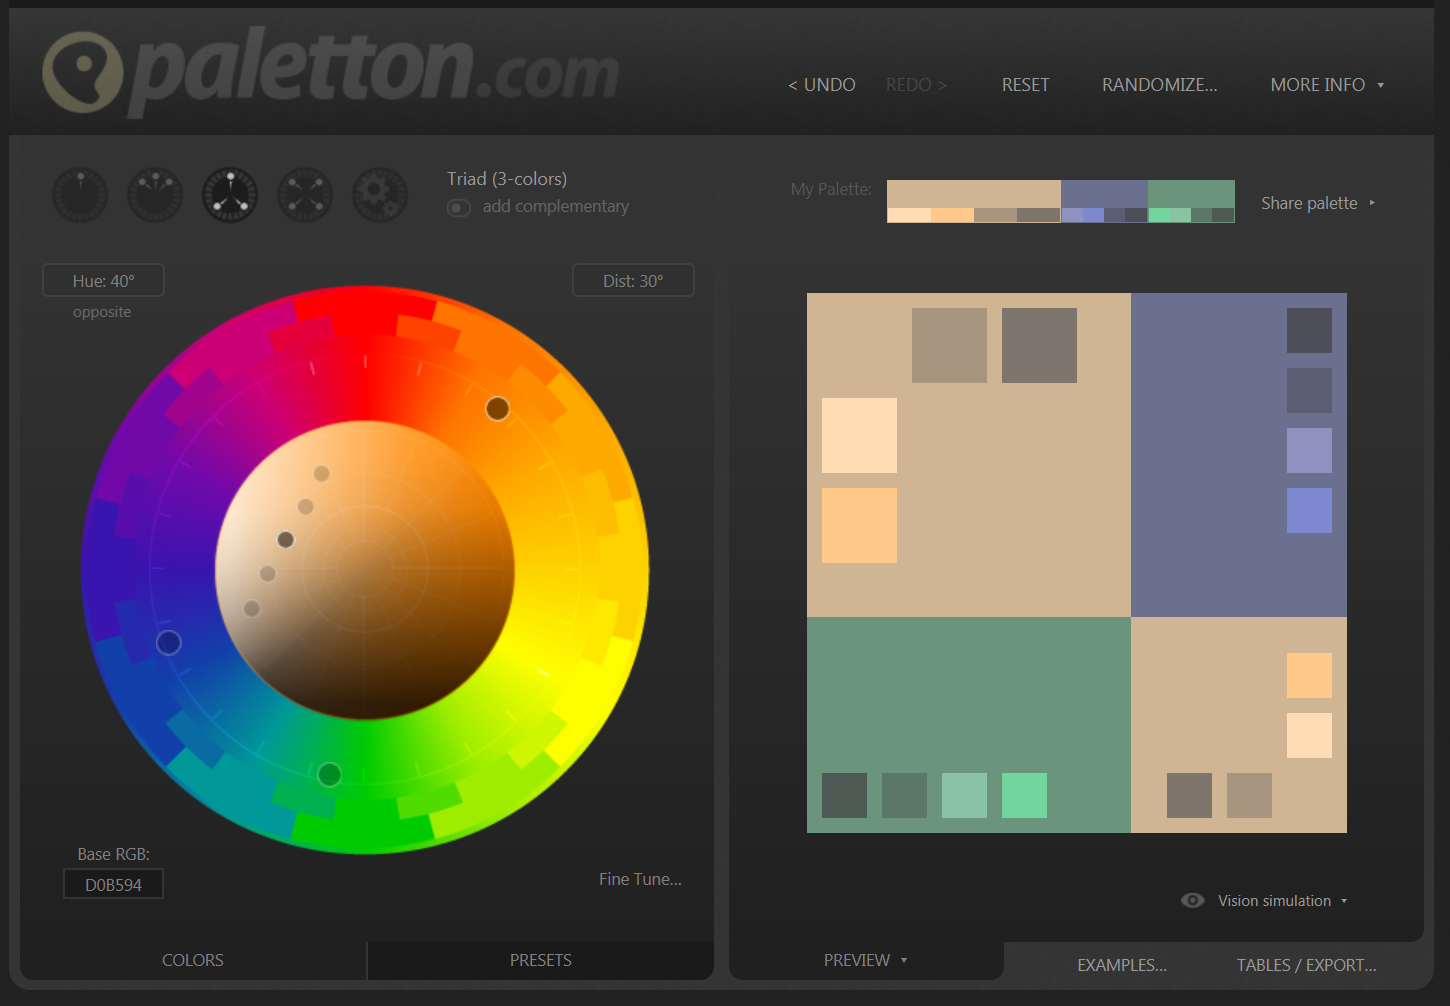
\includegraphics[width=11cm]{assets/palette}
\end{center}

\end{frame}

\begin{frame}

\begin{center}
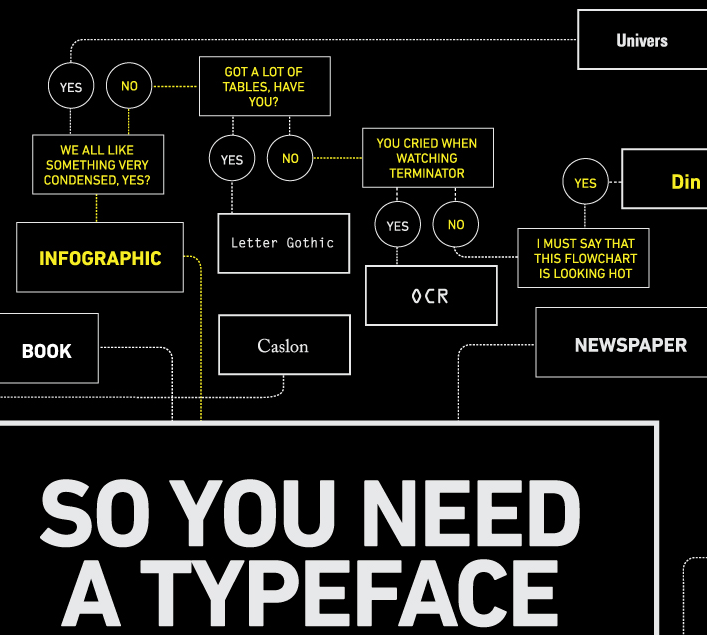
\includegraphics[width=8cm]{assets/crop}
\end{center}


\end{frame}



\begin{frame}

\frametitle{Good engineering and good design go hand in hand.}

According to Dieter Rams:
\begin{enumerate}
\item Is innovative.
\item Makes a product useful.
\item Is aesthetic.
\item Makes a product understandable.
\item Is unobtrusive.
\item Is honest.
\item Is long-lasting.
\item Is thorough down to the last detail.
\item Is environmentally friendly.
\item Involves as little design as possible.
\end{enumerate}

To learn more about the tradition of industrial design: \\ \url{https://www.vitsoe.com/gb/about/good-design}.

\end{frame}

% ---------------------------------

\bibliographystyle{alpha}
\nobibliography{references}

\end{document}